\documentclass[11pt,a4paper]{article}

% ==============================================================================
% PACKAGES
% ==============================================================================
\usepackage[utf8]{inputenc}
\usepackage[margin=1in]{geometry}
\usepackage{amsmath,amssymb}
\usepackage{graphicx}
\usepackage{cite}
\usepackage{booktabs}
\usepackage{enumitem}
\usepackage{float}
\usepackage{caption}
\usepackage{subcaption}
\usepackage{titlesec}
\usepackage{setspace}
\usepackage{xcolor}

% Hyperlink configuration
\usepackage{hyperref}
\hypersetup{
    colorlinks=true,
    linkcolor=black,
    citecolor=blue,
    urlcolor=blue
}

% Image search path: looks in root, current dir, and images folder
\graphicspath{{./}{images/}{assets/}{assets/changes/}}

% ==============================================================================
% SECTION FORMATTING (Matches IEEE / Academic PDF Style)
% ==============================================================================
% Section format: "III. METHODOLOGY"
\renewcommand{\thesection}{\Roman{section}}
\renewcommand{\thesubsection}{\Alph{subsection}}
\renewcommand{\thesubsubsection}{\arabic{subsubsection}}

\titleformat{\section}
  {\normalfont\Large\bfseries\centering}{\thesection.}{0.5em}{\MakeUppercase}

\titleformat{\subsection}
  {\normalfont\large\bfseries}{\thesubsection.}{0.5em}{}

\titleformat{\subsubsection}
  {\normalfont\normalsize\bfseries}{\thesubsubsection.}{0.5em}{}

% Set paragraph spacing for comfortable reading and editing
\setlength{\parskip}{0.6em}
\setlength{\parindent}{0pt}

% Clean workflow arrow box style
\newcommand{\workflowbox}[1]{%
  \begin{center}
    \fcolorbox{gray!30}{gray!5}{%
      \parbox{0.94\columnwidth}{\centering\small\sffamily #1}%
    }
  \end{center}
}

% ==============================================================================
% DOCUMENT BEGIN
% ==============================================================================
\begin{document}

% Manually setting section counter to 3 for Section III
\setcounter{section}{2}
\section{Methodology}
\label{sec:methodology}

Dark patterns can appear in different parts of a webpage, including its text, interface structure, and visual presentation \cite{mathur2019, aidui2023, dpsentinel2024, gray2023}. Therefore, automated detection requires a system that can examine these different forms of information during webpage use. To address this need, we propose \textbf{DarkSight}, a client-side browser extension for detecting and responding to dark patterns during browsing. DarkSight combines text-based, structural, and image-based detection methods and applies a user-selected countermeasure when a dark pattern is detected. Unlike approaches that mainly perform detection after webpages have been collected for offline analysis, DarkSight performs the detection within the user's browser and provides a response on the same webpage.

% ------------------------------------------------------------------------------
\subsection{System Overview}
\label{subsec:system_overview}

DarkSight follows a sequential workflow consisting of \textbf{data collection}, \textbf{dark pattern detection}, and \textbf{countermeasure application}. First, the extension collects the information required for detection from the current webpage. This includes visible text, visual properties and positions of webpage elements, and an image of the visible webpage. The collected information is then processed by the appropriate detection methods. Text is first checked using predefined linguistic patterns, while text that cannot be identified at this stage is analyzed by a local language model. In parallel, the visual presentation of webpage elements is examined using structural analysis, and the webpage screenshot is analyzed to identify visual patterns that cannot be identified from webpage structure alone. When a dark pattern is confirmed, the result is passed to the countermeasure component, which applies the protection mode selected by the user.

Fig.~\ref{fig:architecture} presents the overall architecture of DarkSight and shows the flow from webpage data collection to dark pattern detection and countermeasure application.

\begin{figure}[H]
    \centering
    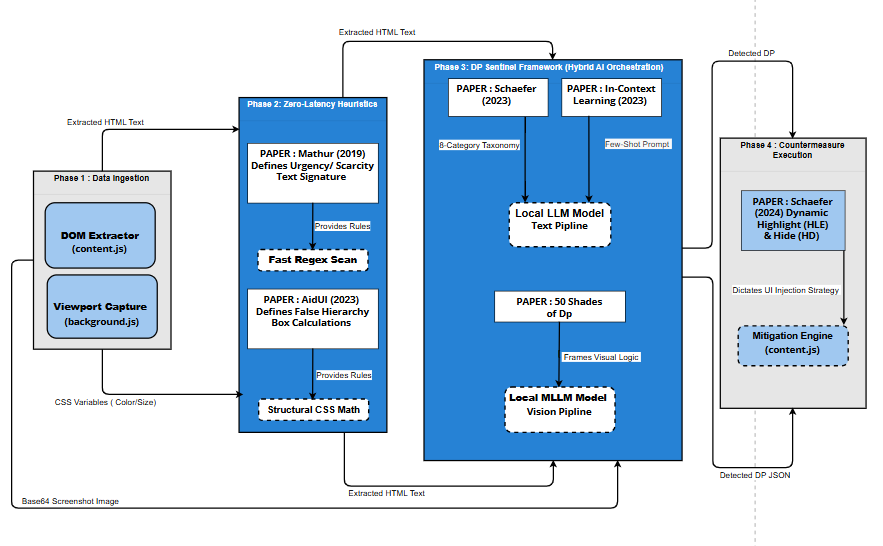
\includegraphics[width=\linewidth]{fig1_architecture.png}
    \caption{Overall architecture and workflow of DarkSight.}
    \label{fig:architecture}
\end{figure}

% ------------------------------------------------------------------------------
\subsection{Webpage Data Collection}
\label{subsec:data_collection}

The first stage of DarkSight collects the information required by the detection methods. The extension examines the current webpage and identifies elements that are visible to the user. Elements that are not displayed or do not have a visible area are excluded to reduce unnecessary processing. For each visible element, DarkSight collects its text and relevant visual properties, including its size, position, and displayed colors.

In addition to webpage element information, DarkSight captures an image of the visible webpage after the page has finished loading. This image provides information that may not be available from the webpage structure, such as dark patterns presented inside images or other graphical content. To avoid repeated image processing when webpage content changes, the screenshot is captured once after the initial page load.

The collected information is then provided to the detection stages according to the type of information required. Text is processed by the textual detection pipeline, webpage element information is used for structural analysis, and the captured webpage image is used for image-based analysis.

% ------------------------------------------------------------------------------
\subsection{Dark Pattern Detection}
\label{subsec:detection}

DarkSight uses three detection levels to examine different forms of dark patterns. The first level identifies text that directly matches predefined patterns. The second level uses a local language model to analyze text that requires further interpretation. The third level examines the visual presentation of webpage elements and the overall webpage image.

These detection methods are based on previous research and adapted for use in a client-side browser extension. Mathur et al.~\cite{mathur2019} provide the basis for the initial text-based detection, Sch\"afer~\cite{schaefer2023} provides the textual dark pattern categories used for language-model analysis, AidUI~\cite{aidui2023} provides the structural analysis approach, and DP Sentinel~\cite{dpsentinel2024} provides the basis for spatial visual analysis. The visual pattern categories used for image-based analysis are based on \textit{50 Shades of Deceptive Patterns}~\cite{gray2023}.

\subsubsection{Tier 1: Linguistic Pattern Detection}
\label{subsubsec:tier1}

The first detection stage checks webpage text against predefined linguistic patterns associated with known dark patterns. This stage is based on the findings of Mathur et al.~\cite{mathur2019}, which identified common dark patterns through a large-scale study of shopping websites.

DarkSight currently checks for four types of textual patterns:
\begin{itemize}[leftmargin=1.5em]
    \item \textbf{Urgency}, such as messages indicating that an offer will expire soon.
    \item \textbf{Scarcity}, such as claims that only a small number of products remain.
    \item \textbf{Social proof}, such as messages stating that many users are currently viewing an item.
    \item \textbf{Fake discount}, such as misleading reference or crossed-out prices.
\end{itemize}

These patterns are checked directly using predefined regular expressions. When the text clearly matches one of these patterns, it can be identified without using the language model. Text that does not match these predefined patterns is passed to the next detection stage for further analysis.

Thus, Tier~1 provides the initial text-based check and reduces the amount of text that needs further model-based analysis.

\subsubsection{Tier 2: Local LLM-Based Text Analysis}
\label{subsubsec:tier2}

Not all dark patterns can be identified using fixed linguistic patterns. A webpage may use different wording to create pressure or influence a user's decision without using a known phrase. Therefore, text that is not identified in Tier~1 is passed to a local \textbf{DeepSeek-R1 1.5B} language model for further analysis.

The local model is guided by a structured prompt based on the textual dark pattern categories proposed by Sch\"afer~\cite{schaefer2023}. The prompt provides the model with the categories and examples needed to analyze the input consistently. The use of examples and structured instructions follows the in-context learning approach described by Sazid et al.~\cite{sazid2023}.

The resulting process is:
\workflowbox{Webpage text $\;\longrightarrow\;$ Tier 1 pattern check $\;\longrightarrow\;$ if not identified $\;\longrightarrow\;$ local LLM analysis $\;\longrightarrow\;$ detection result}

This allows DarkSight to handle both directly recognizable text patterns and cases where understanding the meaning of the text is necessary.

\subsubsection{Tier 3: Visual Analysis}
\label{subsubsec:tier3}

Some dark patterns are mainly expressed through the visual presentation of an interface rather than its text. DarkSight therefore uses two visual analysis methods: \textbf{structural analysis of webpage elements} and \textbf{image-based analysis of the visible webpage}.

\paragraph{3.1 Structural Visual Analysis}
The first visual method examines related interactive elements within the same part of a webpage. In this work, related interactive elements are referred to as \textit{sibling elements}, meaning elements that provide different choices within the same interface area, such as an \textbf{Accept} button and a \textbf{Decline} option.

DarkSight adopts the structural analysis approach proposed by AidUI~\cite{aidui2023} to identify cases where one choice is made visually more prominent than another. For example, an Accept button may have a larger size or stronger visual contrast than a Decline option, making the two choices appear unequal to the user.

For each group of sibling interactive elements, DarkSight compares their visible area and visual contrast. The area comparison considers the relative size of the elements, while the contrast comparison considers how clearly each element appears against its background. These two measurements are considered separately following the structural analysis approach used in AidUI~\cite{aidui2023}.

DarkSight uses the decision threshold adopted from this approach to identify sufficient visual difference between the elements. This also allows the system to detect cases where an option is visually suppressed through lower contrast even when the sizes of the two elements are similar.

\paragraph{3.2 Image-Based Visual Analysis}
Some dark patterns may appear in graphical content or complex webpage regions that cannot be adequately analyzed through webpage elements alone. Examples include patterns contained within images, banners, or visually complex interface regions.

To handle these cases, DarkSight analyzes the captured webpage image using a local \textbf{Qwen2.5-VL} multimodal model. The model is guided by the visual dark pattern categories described in \textit{50 Shades of Deceptive Patterns}~\cite{gray2023}.

The model identifies the location of a suspected dark pattern in the screenshot and returns its position as a bounding box. DarkSight then converts this position from the screenshot coordinates to the corresponding position in the current browser viewport. This allows the detected region to be linked to the correct location on the webpage and used by the countermeasure component.

The overall process is:
\workflowbox{Webpage screenshot $\;\longrightarrow\;$ visual analysis $\;\longrightarrow\;$ detected region $\;\longrightarrow\;$ webpage position $\;\longrightarrow\;$ countermeasure}

The spatial analysis process follows the approach presented by DP Sentinel~\cite{dpsentinel2024}, while the visual pattern categories are based on \cite{gray2023}.

% ------------------------------------------------------------------------------
\subsection{Countermeasure Application}
\label{subsec:countermeasures}

Detection alone does not change the user's experience of a dark pattern. Therefore, after a dark pattern is detected, DarkSight applies a countermeasure according to the user's selected protection mode. The countermeasure design is based on the mitigation concepts presented by Sch\"afer et al.~\cite{schaefer2024}.

Fig.~\ref{fig:countermeasure} presents the countermeasure workflow of DarkSight.

\begin{figure}[H]
    \centering
    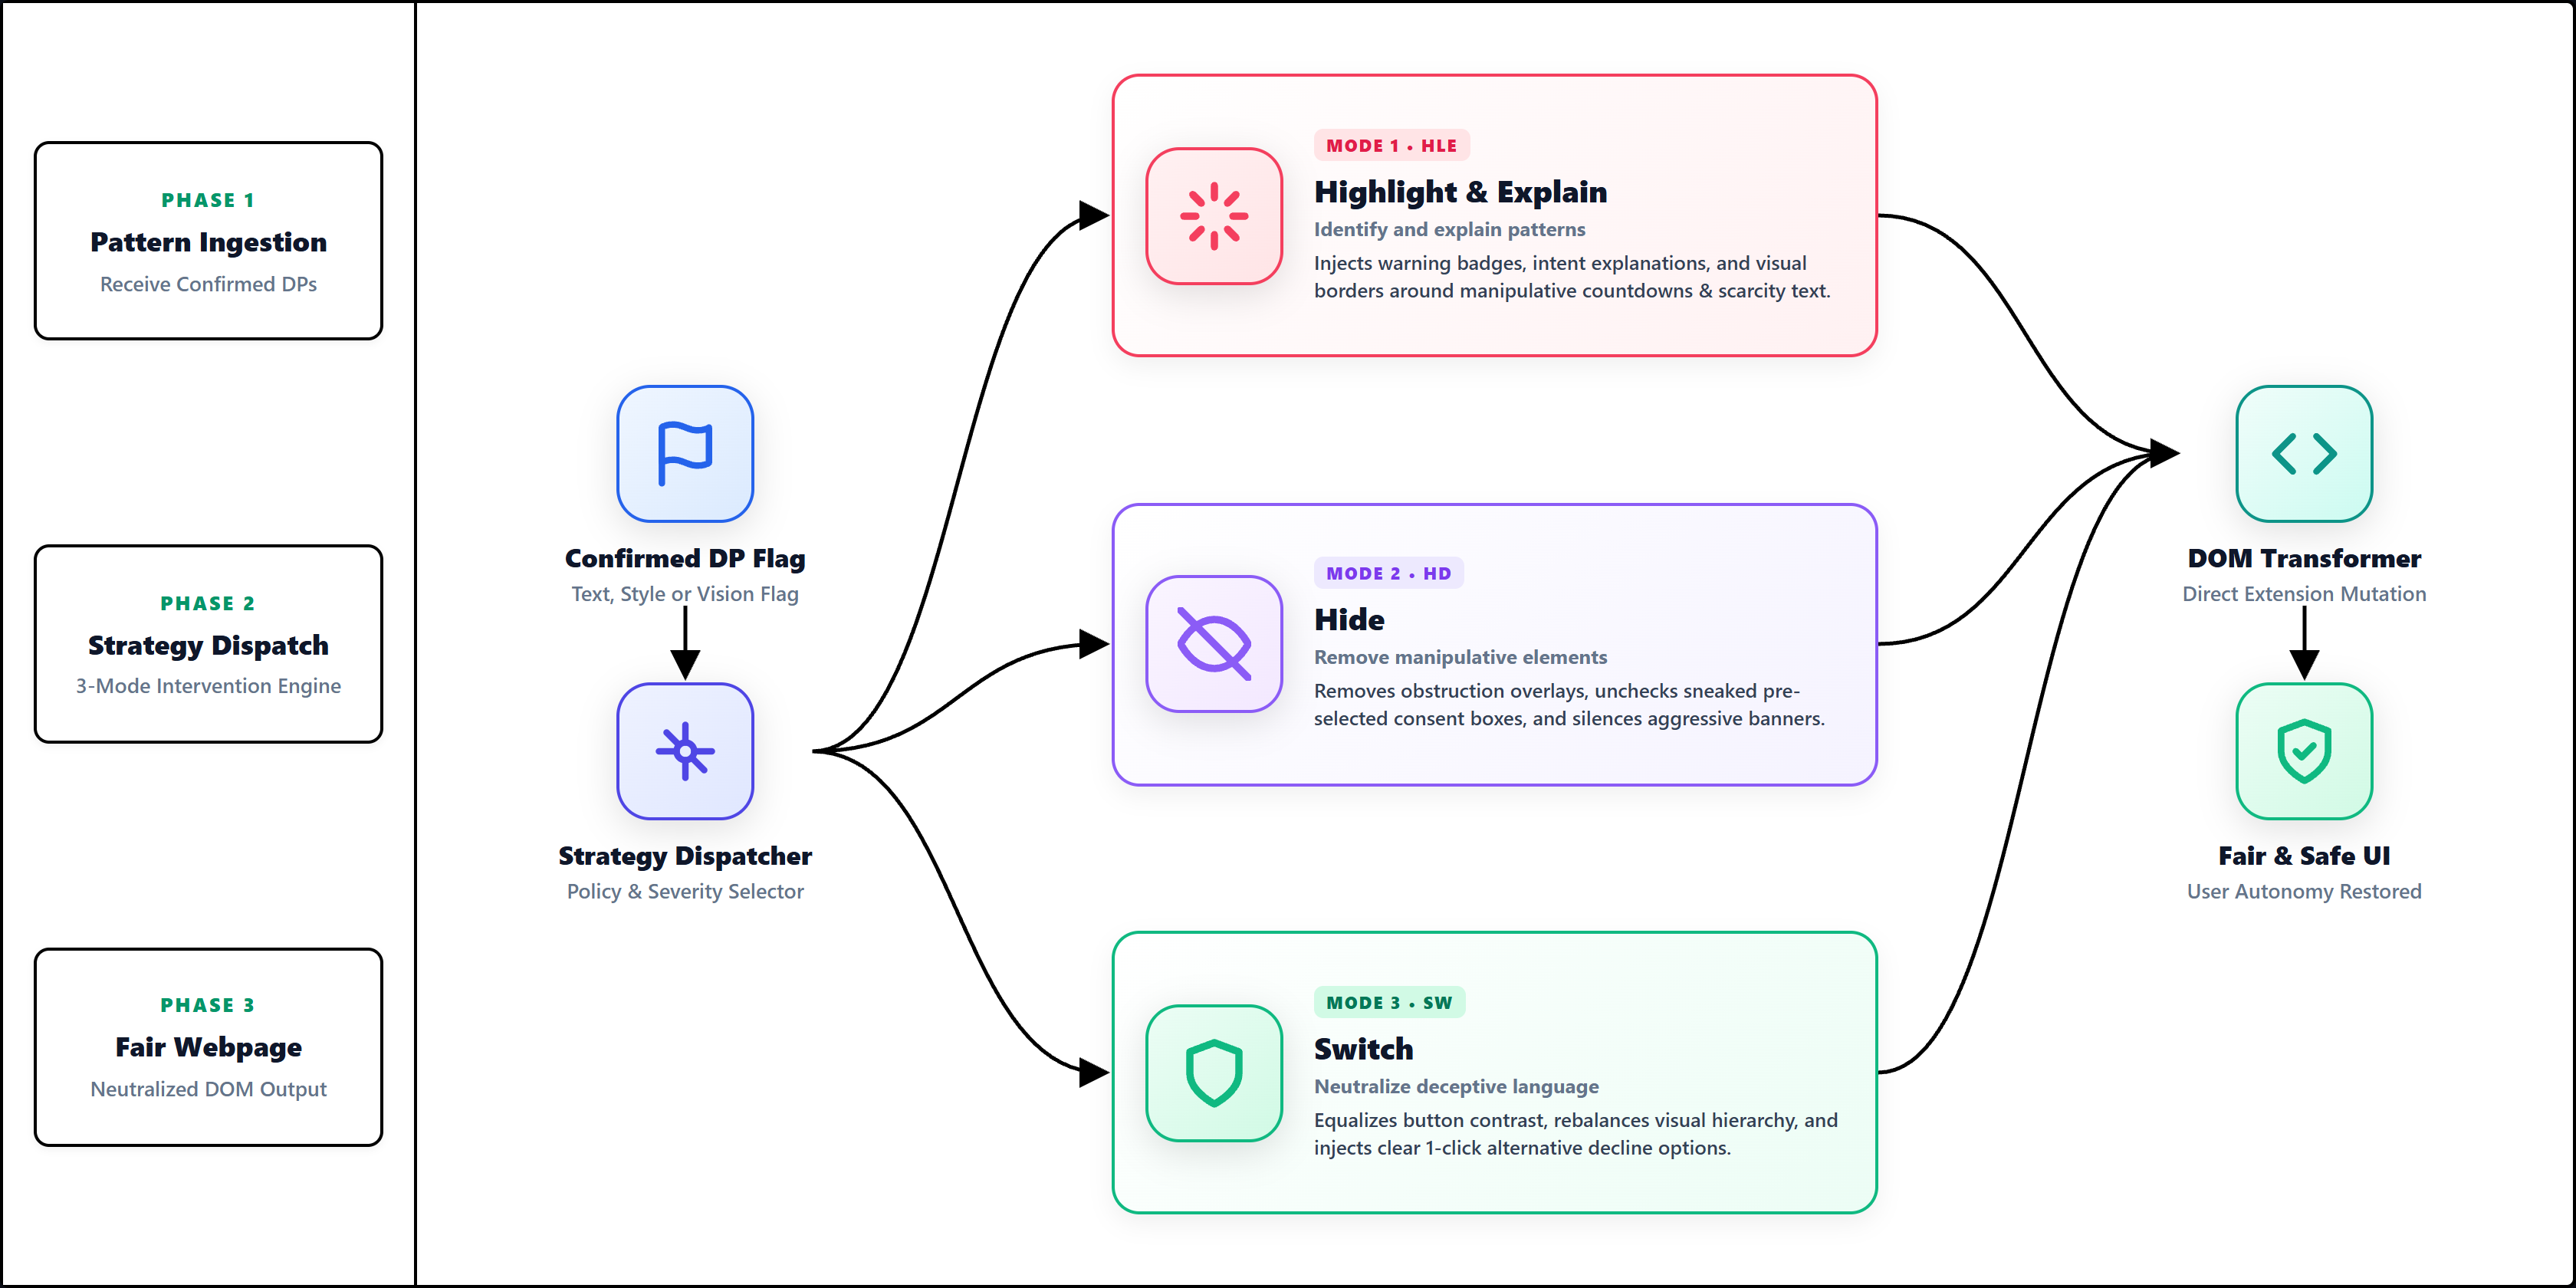
\includegraphics[width=\linewidth]{fig2_countermeasures.png}
    \caption{Countermeasure architecture of DarkSight.}
    \label{fig:countermeasure}
\end{figure}

The countermeasure process consists of three steps: \textbf{detection result preparation}, \textbf{countermeasure selection}, and \textbf{webpage modification}.

\subsubsection{Detection Result Preparation}
The results produced by the textual and visual detection stages are converted into a common format before they are passed to the countermeasure component. This keeps the detected pattern and its target webpage element together so that the same countermeasure process can be used regardless of which detection method identified the pattern.

This step provides a common input for the countermeasure selection process.

\subsubsection{Countermeasure Selection}
DarkSight provides three countermeasure modes. The selected mode determines how a detected dark pattern is presented to the user.

\paragraph{Mode 1: Highlight and Explain (HLE)}
In HLE mode, the detected webpage element is highlighted and an explanation is provided to the user. The explanation identifies the detected dark pattern and helps the user understand why the element was flagged. The original webpage function remains available.

\paragraph{Mode 2: Hide (HD)}
In HD mode, the detected element is hidden from the webpage. This mode is intended for elements that the user does not want to see, such as artificial countdown messages, stock messages, or social-proof notifications.

\paragraph{Mode 3: Switch (SW)}
In SW mode, DarkSight changes misleading content into a more neutral presentation. For textual patterns, high-pressure wording can be replaced with a neutral message. For visually unequal choices, the visual difference between the choices can also be reduced.

Therefore, the three modes provide different levels of user control:
\begin{center}
\begin{tabular}{r c l}
\textbf{HLE} & $\longrightarrow$ & show and explain \\
\textbf{HD}  & $\longrightarrow$ & hide \\
\textbf{SW}  & $\longrightarrow$ & change to a more neutral presentation \\
\end{tabular}
\end{center}

\subsubsection{Webpage Modification}
After the countermeasure mode is selected, DarkSight applies the required change to the detected webpage element. The extension modifies only the relevant element while keeping the normal functions of the webpage, such as navigation and checkout interactions, available.

The complete countermeasure flow is therefore:
\workflowbox{Detected dark pattern $\;\longrightarrow\;$ prepare detection result $\;\longrightarrow\;$ select user mode $\;\longrightarrow\;$ modify target element $\;\longrightarrow\;$ continue browsing}

% ------------------------------------------------------------------------------
\subsection{Integration of Previous Research}
\label{subsec:integration}

DarkSight builds its methodology by adapting established approaches from previous research to a client-side browser environment. Each work contributes a specific part of the proposed system rather than being used as a complete system.

Mathur et al.~\cite{mathur2019} provide the basis for the initial text-pattern detection. Sch\"afer~\cite{schaefer2023} provides the textual dark pattern categories used by the local language model, while Sazid et al.~\cite{sazid2023} inform the use of structured prompts and examples for model-based detection. The structural analysis method is adopted from AidUI~\cite{aidui2023}. DP Sentinel~\cite{dpsentinel2024} provides the basis for the screenshot-based spatial analysis, and the visual categories are taken from \textit{50 Shades of Deceptive Patterns}~\cite{gray2023}. Finally, the countermeasure approach is based on the mitigation framework presented by Sch\"afer et al.~\cite{schaefer2024}.

DarkSight combines these components into a single browser-based workflow. The main consideration in this integration is that each method is used according to the type of information it can analyze: linguistic patterns are checked from text, semantic cases are analyzed using the local language model, visual differences are examined from webpage structure, and graphical patterns are analyzed from the webpage screenshot. The resulting detections are then brought together before the selected countermeasure is applied.

% ------------------------------------------------------------------------------
\subsection{Local Processing and Privacy}
\label{subsec:privacy}

DarkSight performs the model-based processing locally through Ollama. The DeepSeek-R1 model is used for text analysis, while Qwen2.5-VL is used for image-based analysis. As a result, the webpage information required for these analyses is processed on the user's machine rather than being sent to an external model service.

This client-side design also supports the main goal of DarkSight: detecting dark patterns and applying countermeasures during browsing without requiring the webpage data to be processed by a remote detection service.

% ==============================================================================
% REFERENCES
% ==============================================================================
\begin{thebibliography}{7}

\bibitem{mathur2019}
A.~Mathur, G.~Acar, M.~J.~Friedman, E.~Lucherini, J.~Mayer, M.~Chetty, and A.~Narayanan,
``Dark Patterns at Scale: Findings from a Crawl of 11K Shopping Websites,''
\textit{Proceedings of the ACM on Human-Computer Interaction}, vol.~3, no.~CSCW, pp.~1--32, 2019.

\bibitem{schaefer2023}
M.~Sch\"afer et~al.,
``Taxonomy of Dark Patterns for LLM Analysis,''
2023.

\bibitem{sazid2023}
Y.~Sazid, M.~M.~N.~Fuad, and K.~Sakib,
``Automated Detection of Dark Patterns Using In-Context Learning Capabilities of GPT-3,''
in \textit{2023 30th Asia-Pacific Software Engineering Conference (APSEC)}, IEEE, pp.~241--250, 2023.

\bibitem{aidui2023}
S.~M.~H.~Mansur et~al.,
``AidUI: Toward Automated Recognition of Dark Patterns in User Interfaces via Structural Visual Analysis,''
in \textit{2023 IEEE/ACM 45th International Conference on Software Engineering (ICSE)}, IEEE, 2023.

\bibitem{dpsentinel2024}
``Dark Pattern Sentinel: A Hybrid DOM Heuristics and LLM-Based Real-Time Detection System,''
2024.

\bibitem{gray2023}
C.~M.~Gray, C.~Santos, N.~Bielova, M.~Toth, and D.~Clifford,
``50 Shades of Deceptive Patterns: A Taxonomy of Cognitive Biases in Digital Design,''
\textit{International Journal of Human-Computer Studies}, 2023.

\bibitem{schaefer2024}
M.~Sch\"afer, P.~Preuschoff, and J.~Borchers,
``Fighting Malicious Designs: Towards Visual Countermeasures Against Dark Patterns,''
in \textit{Proceedings of the 2024 CHI Conference on Human Factors in Computing Systems (CHI '24)}, 2024.

\end{thebibliography}

\end{document}
